% Template for ICIP-2019 paper; to be used with:
%          spconf.sty  - ICASSP/ICIP LaTeX style file, and
%          IEEEbib.bst - IEEE bibliography style file.
% --------------------------------------------------------------------------
\documentclass{article}
\usepackage{spconf,amsmath,graphicx}
\usepackage[backend=biber, style=ieee]{biblatex}
\addbibresource{reportRefs.bib}

% Example definitions.
% --------------------
\def\x{{\mathbf x}}
\def\L{{\cal L}}

% Title.
% ------
\title{House Price And Affordability In Regions Of Englanf And Wales}
%
% Single address.
% ---------------
% \name{Author(s) Name(s)\thanks{Thanks to XYZ agency for funding.}}

\name{Junsong Yang}
\address{4274056 \\
psyjy3@nottingham.ac.uk}

\begin{document}
%\ninept
%
\maketitle
%

\section{Introduction}
House price has changes dramatically over the past few years. Such changes are drawing 
attentions as they are leading to housing affordability issues. For example, house price 
in London increased drastically these years, as a result, house price is becoming unaffordable
to most of the residents. Analysis of how the house price changed and 
to what extend the affordability is affected by that changes is provided.

This paper is intended to explore this issue based data about house prices and affordability measurements. 
In general, there are four sections, Initial Question, Data Processing, Information Visualisation and Evaluation.
In Initial Questiions section, issuses related to house prices will be discussed therefore research questions 
will be proposed. As for Data Processing part, information about dataset used in this paper will be briefly 
introduced. Visualisation strategies will be discussed in Information Visualisation section alongside 
data cleaning and transformation, and visual encoding. As for the Evaluation part, justifications of
choice of visual encodings and stragies will be provided and also the general reflection of 
development process.

\section{Initial Questiions}
As mentioned above, the increase of house price lead affordability concerns. A better understanding of 
the house market, and affordability of the locals are necessary to study this issue. For instance, 
how the house price changed and to what extend that change has influenced affordability. Hence 
the research questions are proposed as follow.

\begin{enumerate}
  \item How the mean house price across the regions changed 
  from 2000 onward and Which region has cheapest house.
  \item How the ratio of house price to workplace-based earnings
  changed from 2000 onward and which region has the most affordable
  houses.
  \item How the house price and affordability was affected by the economy crisis in 2008.
\end{enumerate}

% structures of visualisation part (two graphs at least)
% 1 describe graphs 150 -200
% 2 visualisation strategies 150 - 200
% 3 how those graphs anwsered the question 150 -200
% 4 (optional) further question emerged ? 100 -200



\section{Data Processing}

The dataset, obtained from office for national statistics, contains annual data from 1997 to 2018 about 
the median house price across regions of England and Wales, the median gross annual 
earnings based on working place associated with different regions and the ratio of 
median house price to median gross annual earnings.\cite{henretty_2019} \cite{henretty_data_2019}
In each part, only annual data is provided. 

The data is grouped by regions, counties and local authorities. Data of median house price, median 
affordability ratio and lower quartile house price is provided for each group. The affordability ratio 
refers to the ratio of house price to annual gross earnings. In this case the Affordability ratio was 
calculated as the ratio of median house price to annual gross workplace-based earnings. 
(work-based earnings refers the earnings based on where a person work and does not necessarily reveal 
the earnings of the local residents.)

Data cleaning and filtering process is essential for the project as the dataset has quite a few garbage data. 
As those initial questions suggest, data from 2000 to 2018 will be preserved and analysed, therefore, data 
out of this rage will be purged. As the data provided is completed so the missing data problem does not need 
to deal with. Since the data is also consistant, the entity resolution will not be a problem. 

Type conversion is an issue spacifically related to the R programming language. The original data came in 
xls form with the correct type for each category of data. But when loading those data into R, the default 
data type was character. This issue may cause severe problem whrm performing numeric analysis and visualisation. 
Therefore, data of house price, affordability ratio and data indicating time need to be converted into numeric type. 
 


\section{Information Visualisation}



% Below is an example of how to insert images. Delete the ``\vspace'' line,
% uncomment the preceding line ``\centerline...'' and replace ``imageX.ps''
% with a suitable PostScript file name.
% -------------------------------------------------------------------------
\begin{figure}[htb]

\begin{minipage}[b]{1.0\linewidth}
  \centering
  \centerline{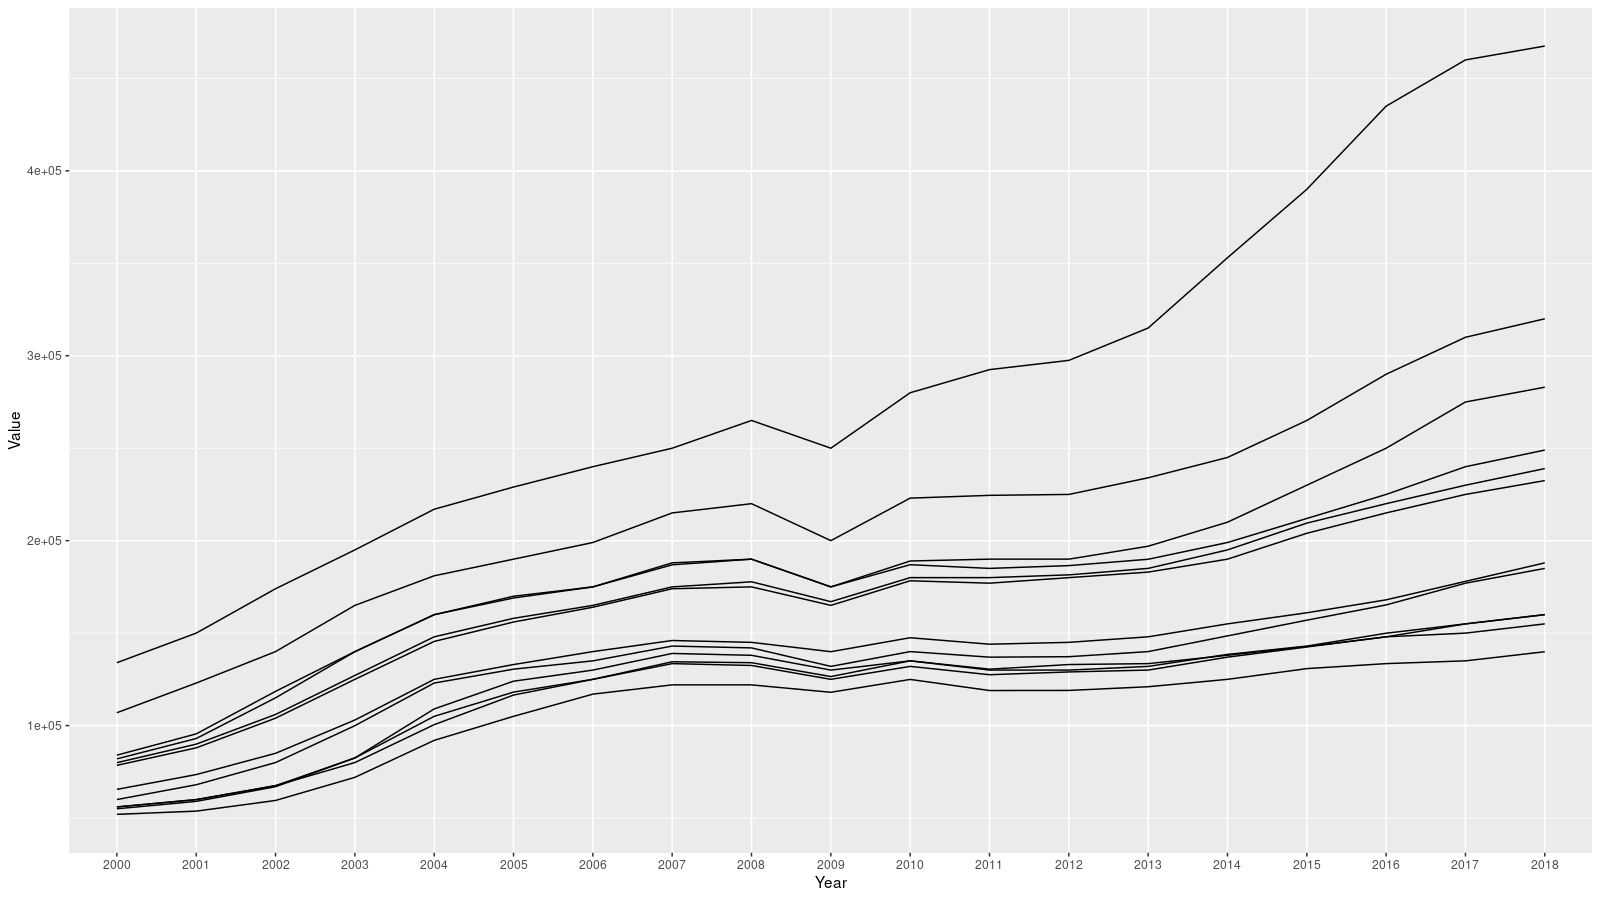
\includegraphics[width=8.5cm]{Q1Geom_line_no_colour}}
%  \vspace{2.0cm}
  \centerline{(a) Result 1}\medskip
\end{minipage}
%
\begin{minipage}[b]{.48\linewidth}
  \centering
  \centerline{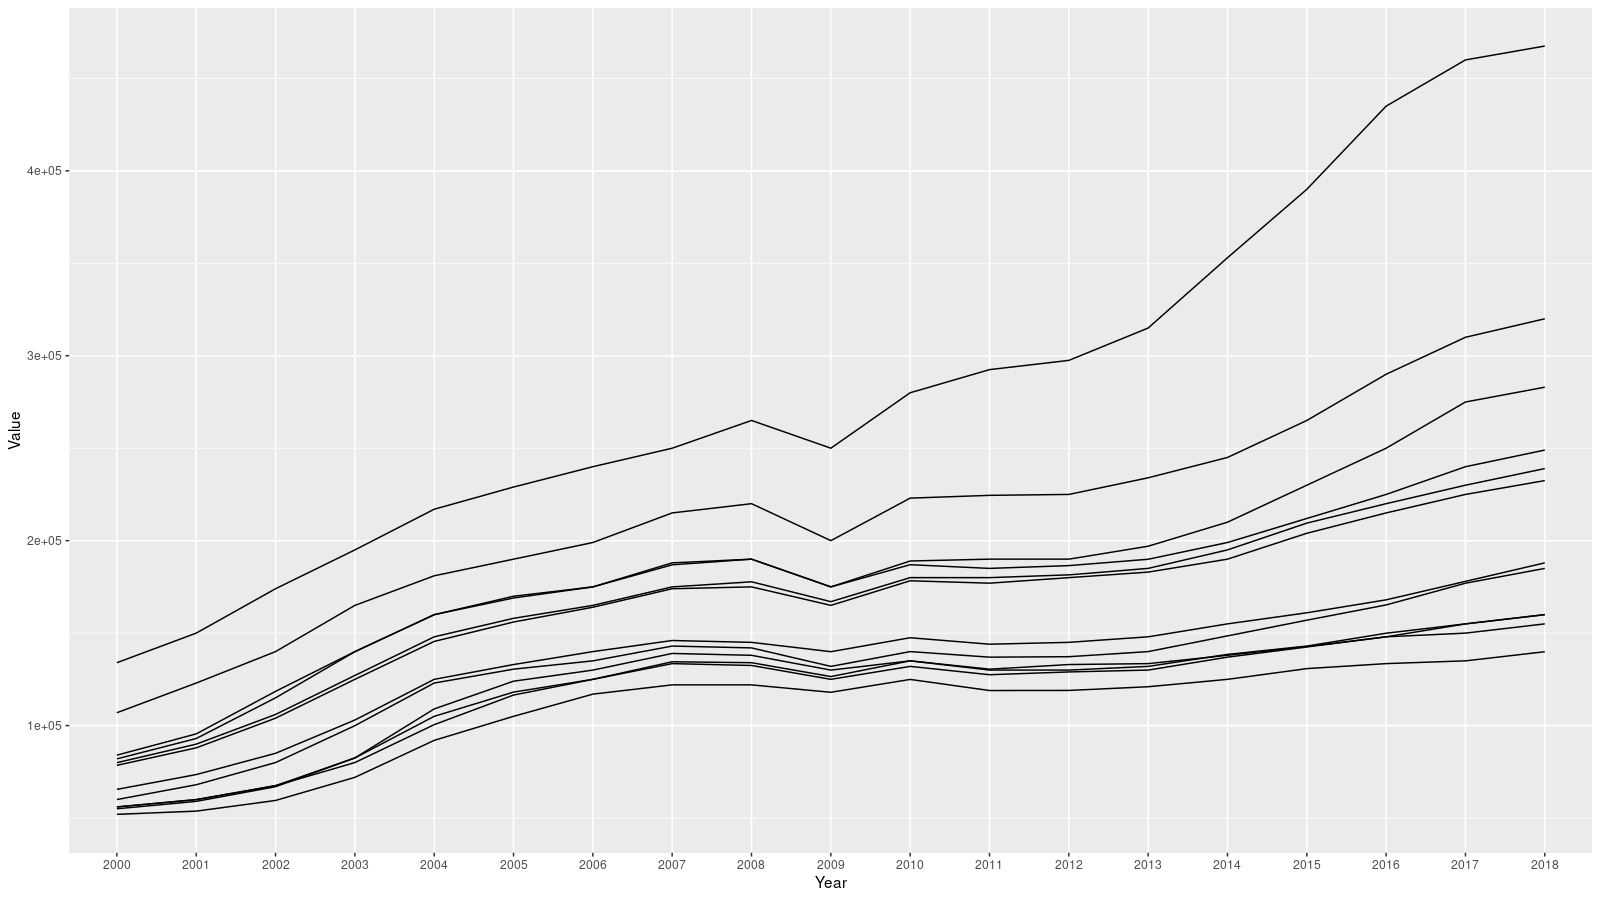
\includegraphics[width=4.0cm]{Q1Geom_line_no_colour}}
%  \vspace{1.5cm}
  \centerline{(b) Results 3}\medskip
\end{minipage}
\hfill
\begin{minipage}[b]{0.48\linewidth}
  \centering
  \centerline{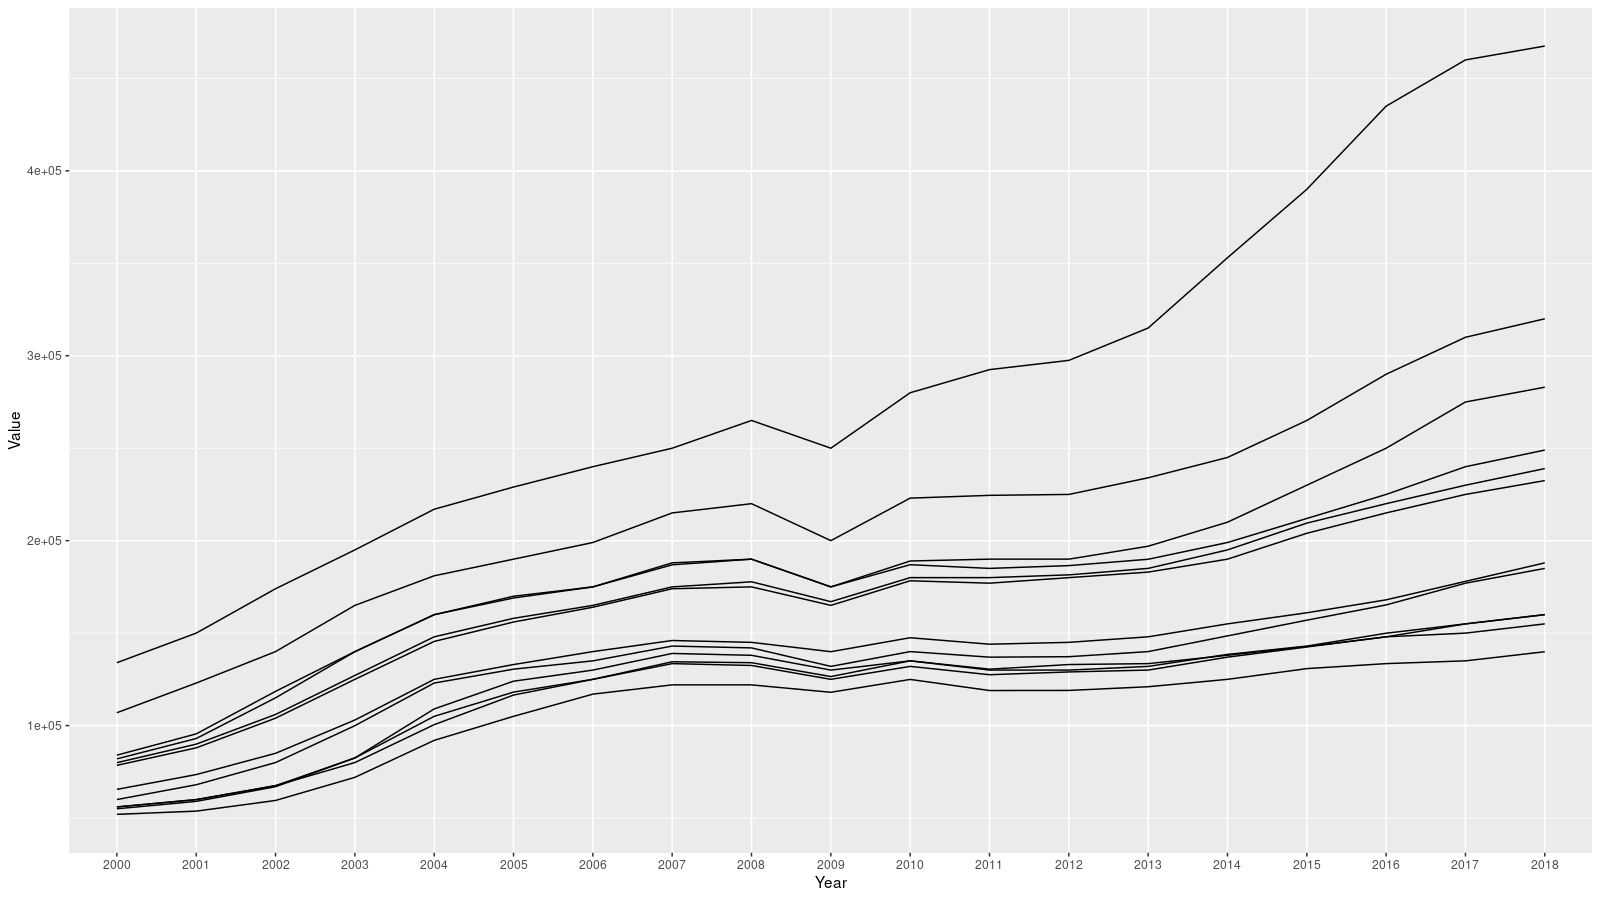
\includegraphics[width=4.0cm]{Q1Geom_line_no_colour}}
%  \vspace{1.5cm}
  \centerline{(c) Result 4}\medskip
\end{minipage}
%
\caption{Example of placing a figure with experimental results.}
\label{fig:res}
%
\end{figure}

\section{Evaluation}
\subsection{Subheadings}
 
\subsubsection{Sub-subheadings}


% To start a new column (but not a new page) and help balance the last-page
% column length use \vfill\pagebreak.
% -------------------------------------------------------------------------
%\vfill
%\pagebreak

\vfill\pagebreak
\printbibliography


\end{document}
